\documentclass[czech]{article}% use option titlepage to get the title on a page of its own.
\usepackage{booktabs}
\usepackage{indentfirst}
\usepackage{listings}
\usepackage{hyperref}
\usepackage{fancyhdr}
\usepackage{a4wide}
\usepackage{dblfloatfix}
\usepackage{float}
\usepackage{upgreek}
\usepackage{graphicx}
\usepackage[table,xcdraw]{xcolor}
\usepackage[czech]{babel}
\usepackage[autostyle=true,czech=quotes]{csquotes}

\renewcommand \thesection {\arabic{section}}
\renewcommand \thesubsection {\thesection.\alph{subsection}}
\renewcommand \thesubsubsection {\thesubsection.\alph{subsubsection}}

\title{Pravděpodobnost a statistika\\
    \large Domácí úkoly 1S-4S\\
    \large Zadání 123}

\author{Martin Pustka} 
\date{\today}

\setlength{\headheight}{12.41254pt}
\pagestyle{fancy}
\fancyhf{}
\lhead{Martin Pustka, PUS0065}
\rhead{Číslo zadání 123}
\chead{Ostrava, AR 2020/2021}
\cfoot{\thepage}

\restylefloat{table}
\restylefloat{figure}

\begin{document}

\maketitle

\noindent
Jméno studenta: Martin Pustka\\
Osobní číslo: PUS0065\\
Jméno cvičícího: Ing. Michal Béreš\\

\begin{table*}[!b]
    \centering
    \begin{tabular}{|l|p{5cm}|p{3cm}|}
        \hline
        & Datum odevzdání & Hodnocení \\
        \hline
        Domácí úkol 1: & & \\
        \hline
        Domácí úkol 2: & & \\
        \hline
        Domácí úkol 3: & & \\
        \hline
        Domácí úkol 4: & & \\
        \hline
        Celkem: & & \\
        \hline
    \end{tabular}
\end{table*}
\newpage
\tableofcontents
\newpage

\noindent
\textbf{Popis datového souboru}
\\\\
\noindent
Běžné zářivky trpí efektem pomalého nabíhání, tedy plného výkonu dosáhnou až po jisté době provozu. Toto chování je ovlivněno okolní teplotou, což v praxi znamená, že v chladném prostředí může zářivkám trvat výrazně déle než dosáhnou maximálního výkonu. 
\\\\
\noindent
Pro test náběhu zářivek na plný světelný výkon bylo vybráno celkem 350 zářivek od čtyř různých výrobců (Amber, Bright, Clear, Dim). Všechny zářivky měly deklarovaný maximální světelný tok 1000 lm. U každé zářivky byl změřen světelný tok po 30 sekundách od zapnutí, nejprve při teplotě 22 °C a poté při teplotě 5°C.
\\\\
\noindent
V souboru ukol\_X.xslx jsou pro každou z testovaných zářivek uvedeny následující údaje:
\begin{itemize}
    \item pořadové číslo zářivky,
    \item výrobce – Amber (A), Bright (B), Clear (C), Dim (D),
    \item naměřený světelný tok v lumenech při okolní teplotě 5°C,
    \item naměřený světelný tok v lumenech při okolní teplotě 22°C.
\end{itemize}

\noindent
\textbf{Obecné pokyny:}
\begin{itemize}
    \item Úkoly zpracujte dle obecně známých typografických pravidel.
    \item Všechny tabulky i obrázky musí být opatřeny titulkem.
    \item Do úkolů nevkládejte tabulky a obrázky, na něž se v doprovodném textu nebudete odkazovat.
    \item Bude-li to potřeba, citujte zdroje dle mezinárodně platné citační normy ČSN ISO 690.
\end{itemize}


\newpage
\section{Úkol 1S}
\subsection{Zadání}
Pomocí nástrojů explorační analýzy analyzujte světelný tok zářivek výrobce Amber po 30 sekundách od zapnutí při teplotách 5°C a 22°C. Data vhodně graficky prezentujte (krabicový graf, histogram, q-q graf) a doplňte následující tabulky a text.

Výsledky popisné statistiky lze vidět v tabulce \ref{tab:statAmber} a na obrazcích \ref{fig:Boxploty},\ref{fig:Histogram5},\ref{fig:Histogram22},\ref{fig:QQ5} a \ref{fig:QQ22}.
Boxplot obsahuje odlehlá pozorování, ostatní grafy jsou bez odlehlých pozorování.

\subsection{Tabulkové řešení}
\noindent
\begin{table}[H]
	\centering
	\caption{Světelný tok (lm) zářivek Amber v závislosti na teplotě (souhrnné statistiky)}
	\label{tab:statAmber}
	\begin{tabular}{lccl|cc}
        \hline
        \rowcolor[HTML]{F2F2F2} 
        \multicolumn{2}{l}{\cellcolor[HTML]{F2F2F2}Světelný tok zářivek Amber (lm)} & & & \multicolumn{2}{l}{\cellcolor[HTML]{F2F2F2}Po   odstranění odlehlých pozorování} \\
        \rowcolor[HTML]{F2F2F2} 
        \hline
        & 5°C             & 22°C             && 5°C                                    & 22°C                                    \\
        \hline
        rozsah souboru           & 71,0                        & 71,0                         &  & 70,0                                   & 71,0                                    \\
        minimum                  & 750,0                       & 755,8                        &  & 750,0                                  & 755,8                                   \\
        dolní kvartil            & 774,0                       & 774,0                        &  & 773,4                                  & 774,0                                   \\
        medián                   & 797,8                       & 801,9                        &  & 797,4                                  & 801,9                                   \\
        průměr                   & 797,5                       & 797,6                        &  & 795,6                                  & 797,6                                   \\
        horní kvartil            & 818,3                       & 819,6                        &  & 817,9                                  & 819,6                                   \\
        maximum                  & 927,4                       & 875,1                        &  & 882,9                                  & 875,1                                   \\
        směrodatná odchylka      & 30,5                        & 25,8                         &  & 26,4                                   & 25,8                                    \\
        variační koeficient (\%) & 3,8                         & 3,2                          &  & 3,3                                    & 3,2                                     \\
        šikmost                  & 1,2                         & 0,1                          &  & 0,3                                    & 0,1                                     \\
        špičatost                & 3,4                         & -0,5                         &  & 0,0                                    & -0,5                                    \\
        \hline
        \rowcolor[HTML]{F2F2F2} 
        \multicolumn{3}{l}{\cellcolor[HTML]{F2F2F2}Identifikace   odlehlých pozorování – vnitřní hradby}                 &&   &                                         \\
        \hline
        dolní mez                & 707,6                       & 705,6                        &  & 706,6                                  & 705,6                                   \\
        horní mez                & 884,7                       & 888,0                        &  & 884,6                                  & 888,0                                   \\
        \hline
        \end{tabular}
\end{table}

\newpage
\subsection{Grafické řešení}

\begin{figure}[H]
	\centering
	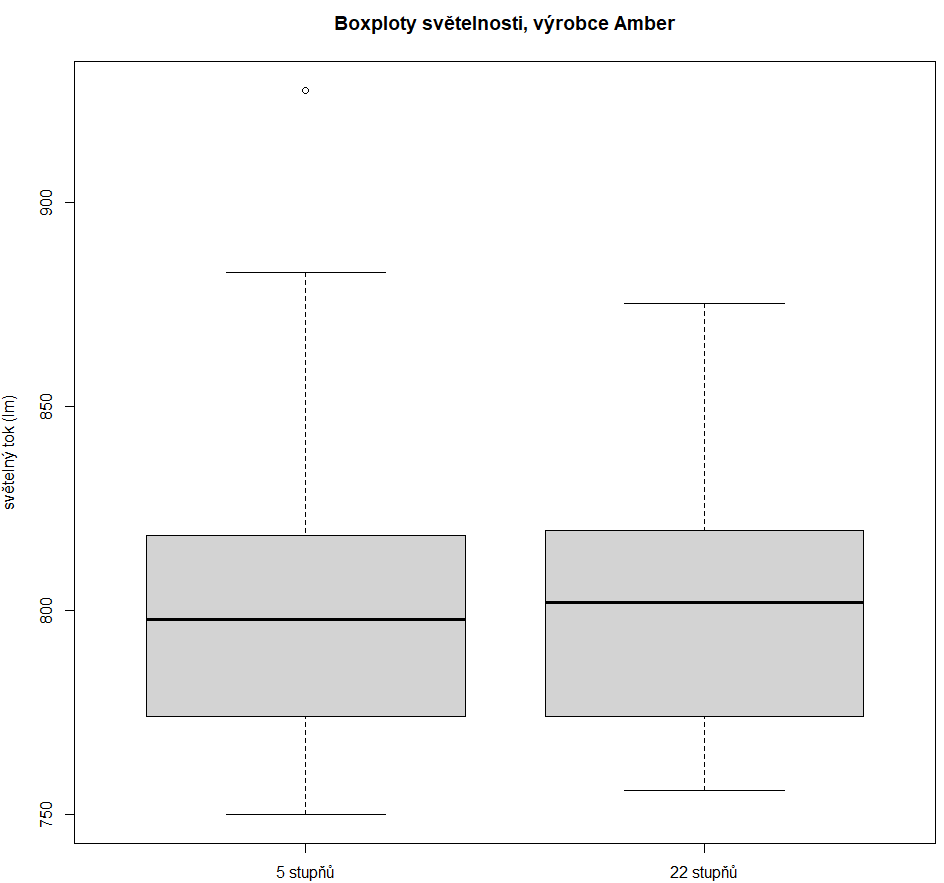
\includegraphics[width=0.6\textwidth]{Figures/Boxploty.png}
	\caption[Boxploty světelnosti, Amber]{Boxploty světelnosti, Amber}
	\label{fig:Boxploty}
\end{figure}

\newpage
\begin{figure}[H]
	\centering
	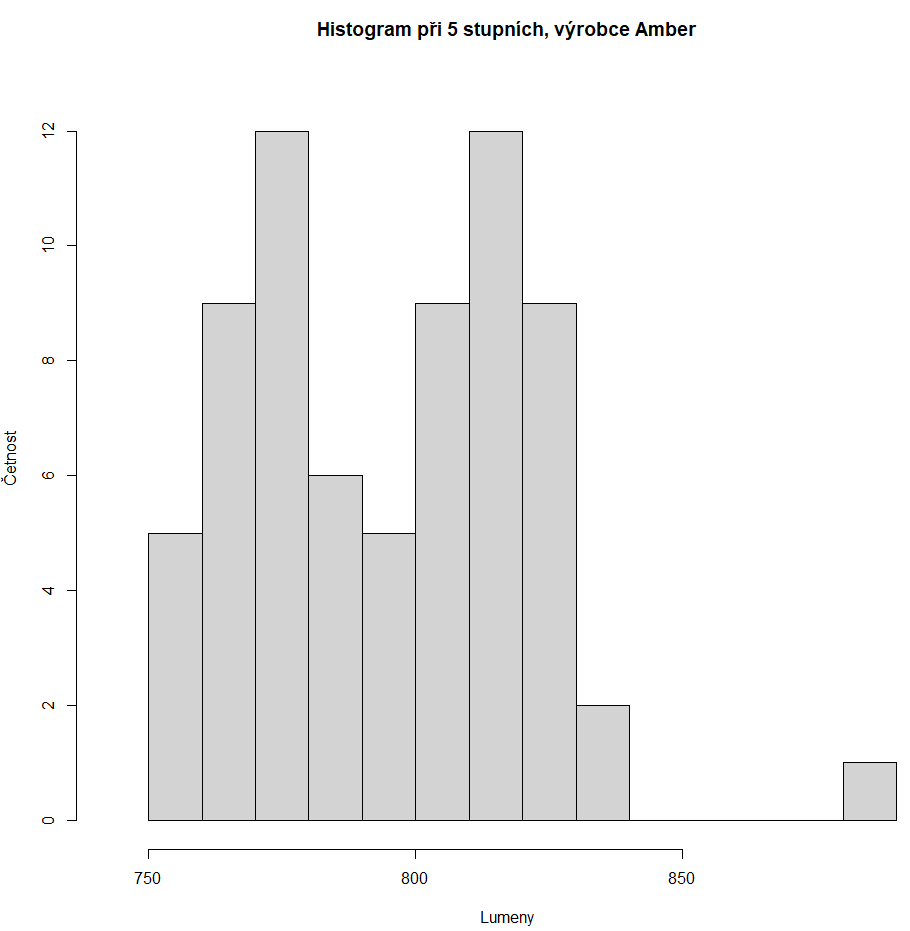
\includegraphics[width=0.6\textwidth]{Figures/Histogram5.png}
	\caption[Histogram světelnosti 5C, Amber]{Histogram světelnosti při 5 stupních, výrobce Amber}
	\label{fig:Histogram5}
\end{figure}

\begin{figure}[H]
	\centering
	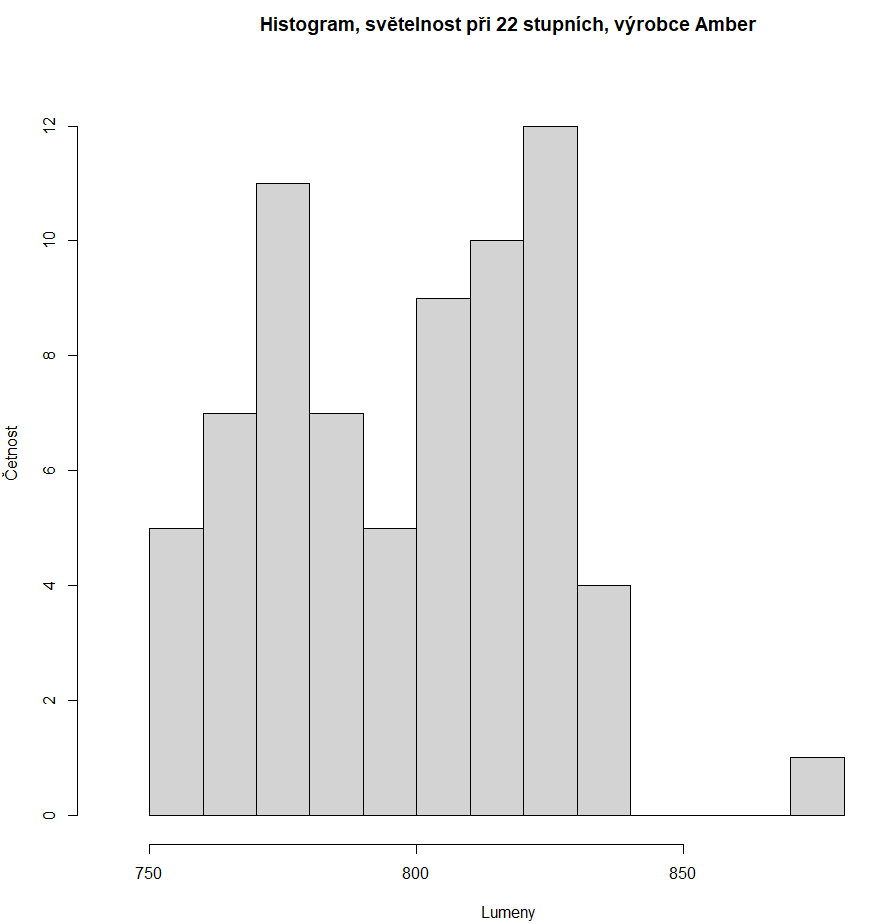
\includegraphics[width=0.6\textwidth]{Figures/Histogram22.png}
	\caption[Histogram světelnosti 22C, Amber]{Histogram světelnosti při 22 stupních, výrobce Amber}
	\label{fig:Histogram22}
\end{figure}

\newpage
\begin{figure}[H]
	\centering
	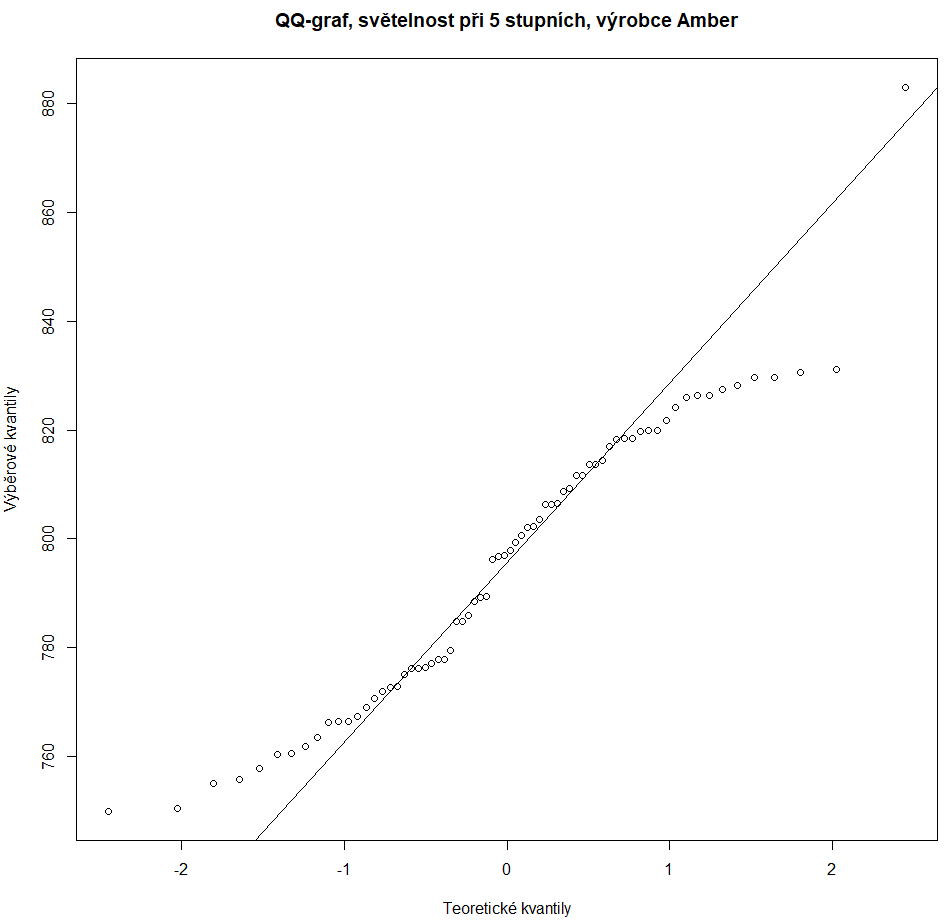
\includegraphics[width=0.6\textwidth]{Figures/QQ5.png}
	\caption[QQ graf světelnosti 5C, Amber]{QQ graf světelnosti při 5 stupních, výrobce Amber}
	\label{fig:QQ5}
\end{figure}

\begin{figure}[H]
	\centering
	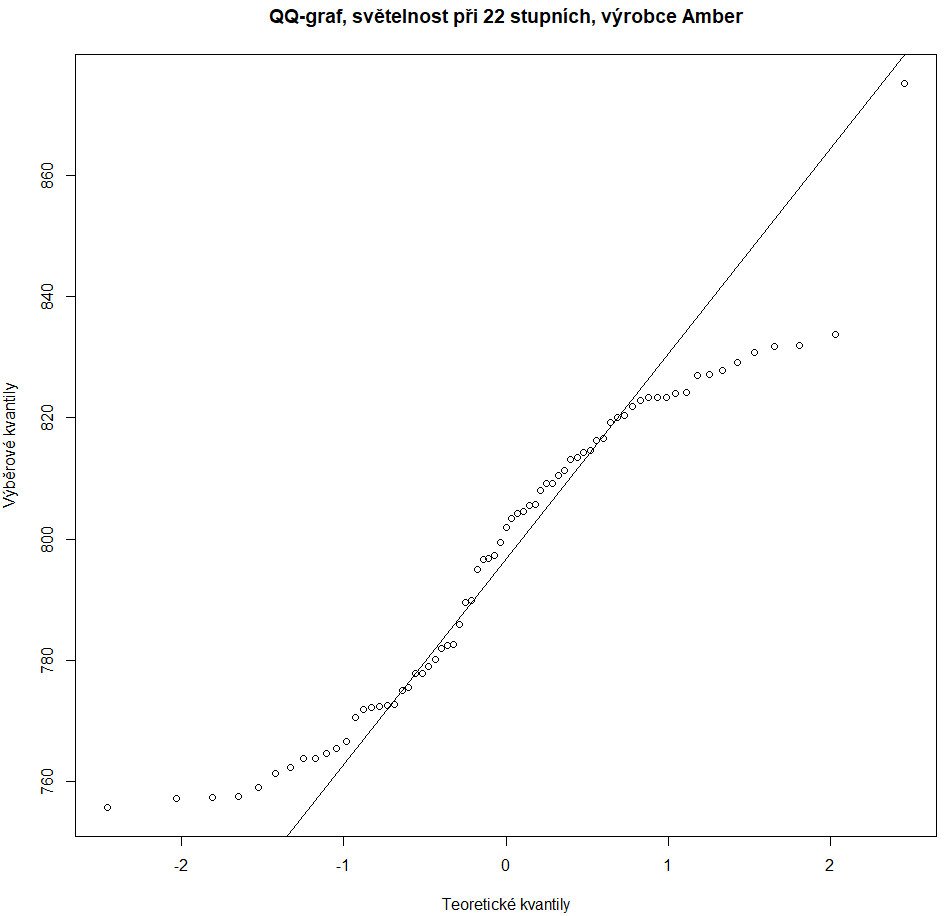
\includegraphics[width=0.6\textwidth]{Figures/QQ22.png}
	\caption[QQ graf světelnosti 5C, Amber]{QQ graf světelnosti při 5 stupních, výrobce Amber}
	\label{fig:QQ22}
\end{figure}

\newpage
\subsection{Textové řešení}

\textbf{Analýza světelného toku zářivek výrobce Amber (po 30 sekundách od zapnutí, při teplotě 5°C)}

Během testu byl měřen světelný tok \textit{71} kusů zářivek výrobce Amber. 
Naměřená světelný tok při teplotě 5°C se pohyboval v rozmezí \textit{750,0} lm až \textit{927,4} lm. 
Světelný tok zářivek č. \textit{27} byl na základě metody vnitřních hradeb identifikován jako 
odlehlé pozorování a nebude zahrnut do dalšího zpracování. Možné příčiny vzniku odlehlých pozorování jsou: \textit{chyby v měření nebo při výrobě}. 
Dále uvedené výsledky tedy pocházejí z analýzy světelný toku \textit{70} kusů zářivek. Jejich průměrný světelný tok byl \textit{795,6} lm, 
směrodatná odchylka pak \textit{26,4} lm. U poloviny testovaných zářivek světelný tok nepřekročil \textit{797,4} lm. 
V polovině měření se světelný tok pohyboval v rozmezí \textit{773,4} lm až \textit{817,9} lm. 
Vzhledem k hodnotě variačního koeficientu (\textit{3,3 \%}) lze analyzovaný soubor považovat za homogenní.\\


\textbf{Analýza světelného toku zářivek výrobce Amber (po 30 sekundách od zapnutí, při teplotě 22°C)}

Během testu byl měřen světelný tok \textit{71} kusů zářivek výrobce Amber. 
Naměřená světelný tok při teplotě 22°C se pohyboval v rozmezí \textit{755,8} lm až \textit{875,1} lm. 
Žádné z měření nebylo identifikováno jako odlehlé pozorování. 
Dále uvedené výsledky tedy pocházejí z analýzy světelný toku \textit{71} kusů zářivek. Jejich průměrný světelný tok byl \textit{797,6} lm, 
směrodatná odchylka pak \textit{25,8} lm. U poloviny testovaných zářivek světelný tok nepřekročil \textit{801,9} lm. 
V polovině měření se světelný tok pohyboval v rozmezí  \textit{774,0} lm až \textit{819,6} lm. 
Vzhledem k hodnotě variačního koeficientu (\textit{3,2} \%) lze analyzovaný soubor považovat za homogenní.\\


\textbf{Ověření normality světelného toku zářivek výrobce Amber po 30 sekundách od zapnutí při teplotě 5°C na základě explorační analýzy}

Na základě grafického zobrazení (viz obrázek \ref{fig:QQ5}) a výběrové šikmosti a špičatosti (výběrová šikmost i špičatost leží v intervalu (-2;2)) 
lze předpokládat, že světelný tok zářivek výrobce Amber při teplotě 5°C má normální rozdělení. Dle pravidla 3$\upsigma$ 
lze tedy očekávat, že přibližně 95 \% zářivek bude mít světelný tok v rozmezí \textit{742,9} lm až \textit{848,3} lm.\\


\textbf{Ověření normality světelného toku zářivek výrobce Amber po 30 sekundách od zapnutí při teplotě 22°C na základě explorační analýzy}

Na základě grafického zobrazení (viz obrázek \ref{fig:QQ22}) a výběrové šikmosti a špičatosti (výběrová šikmost i špičatost leží v intervalu (-2;2)) 
lze předpokládat, že světelný tok zářivek výrobce Amber při teplotě 22°C má normální rozdělení. Dle pravidla 3$\upsigma$ 
lze tedy očekávat, že přibližně 95 \% zářivek bude mít světelný tok v rozmezí \textit{746,0} lm až \textit{849,2} lm.\\



\end{document}